\section{Introduction}
\label{sec:introduction}
Volatility forecasts are sensitive to both the information set and the quantity being predicted. Persistent volatility, nonlinear responses to market conditions, and low-frequency macroeconomic indicators motivate models that combine daily market information with monthly economic policy uncertainty (EPU). Yet an apparent improvement can also reflect predictable residual dynamics, a different loss function, data preparation errors, or numerical optimization behavior. A useful comparison must distinguish these mechanisms rather than treat every lower reported loss as evidence of a better economic model.

This study uses a market-only XGBoost predictor as a first stage and models its realized forecast errors in a second stage. A MIDAS-weighted monthly EPU signal enters alongside a lagged error. A residual-only correction supplies the relevant ablation: it asks whether the EPU component adds predictive information beyond error persistence. The target is a daily squared-return proxy, not high-frequency realized variance. This distinction matters for interpretation and for comparisons with the realized-volatility literature.

ARCH and GARCH model conditional heteroskedasticity directly \citep{Engle1982,Bollerslev1986}. Research on realized volatility uses intraday information to construct more informative ex post measures \citep{AndersenBollerslevDieboldLabys2003}; the HAR framework captures persistence across horizons \citep{Corsi2009}. Here, HAR-style daily, weekly, and monthly features are constructed from daily squared returns, so results should not be described as tests of a full intraday realized-volatility implementation. Extensions such as realized kernels and jump-robust measures are relevant alternatives but are not implemented in this experiment.

News-based EPU indices measure the prevalence of policy-related economic uncertainty in specified sources \citep{BakerBloomDavis2016,DavisLiuSheng2019}. Prior work links EPU to stock-market volatility \citep{LiuZhang2015}, while MIDAS and GARCH-MIDAS provide established methods for combining sampling frequencies \citep{GhyselsSinkoValkanov2007,EngleGhyselsSohn2013}. The present second stage is not GARCH-MIDAS: it corrects a log-target point forecast using a weighted EPU signal and an observed lagged forecast error. EPU is not treated as an exogenous policy shock, and a nonzero fitted coefficient does not identify a causal effect.

XGBoost provides a regularized boosted-tree implementation \citep{ChenGuestrin2016}. Evidence on machine learning in empirical asset pricing \citep{GuKellyXiu2020} motivates nonlinear modeling, but does not by itself establish an advantage for this target or data set. The market-only baseline and its residual-only correction are therefore essential comparisons. Standard HAR and GARCH remain informative, although the benchmark set is not exhaustive.

Evaluation also depends on the forecast target and loss. Proxy-robust loss rankings require conditions on the proxy \citep{Patton2011}; those conditions cannot simply be assumed after nonlinear transformations and numerical floors. Forecast-comparison tests \citep{DieboldMariano1995,ClarkWest2007} are not automatically valid for every estimated, selected, or nested model. Coverage diagnostics \citep{Christoffersen1998} and interval scores \citep{GneitingRaftery2007} reveal properties that point losses omit. Although the interval construction uses conformal-style order statistics, it is not an implementation of EnbPI and does not inherit that method's guarantees \citep{Vovk2005,ShaferVovk2008,Lei2018,XuXie2021}.

The study has three practical aims. First, it reconciles archived data, configurations, and numerical results. Second, it reassesses the incremental EPU component using a stable solver, a residual ablation, and multiple losses. Third, it evaluates interval behavior and compares markets while preserving the distinction between current and historical results. The resulting contribution is an auditable empirical reanalysis, not a claim to invent MIDAS, boosting, error correction, or conformal prediction. The literature comparison is selective rather than a systematic review, and no priority claim is made.

The design is retrospective. Historical results were already known before the current revision, and the additional markets are not untouched external validation samples. Data-snooping concerns therefore remain even when the revised estimation and validation rules are fixed before inspecting the newly computed test results \citep{LoMacKinlay1990,HarveyLiuZhu2016}. Confirmatory evidence would require a locked design and new observations with documented real-time information availability.

\begin{figure}[htbp]
\centering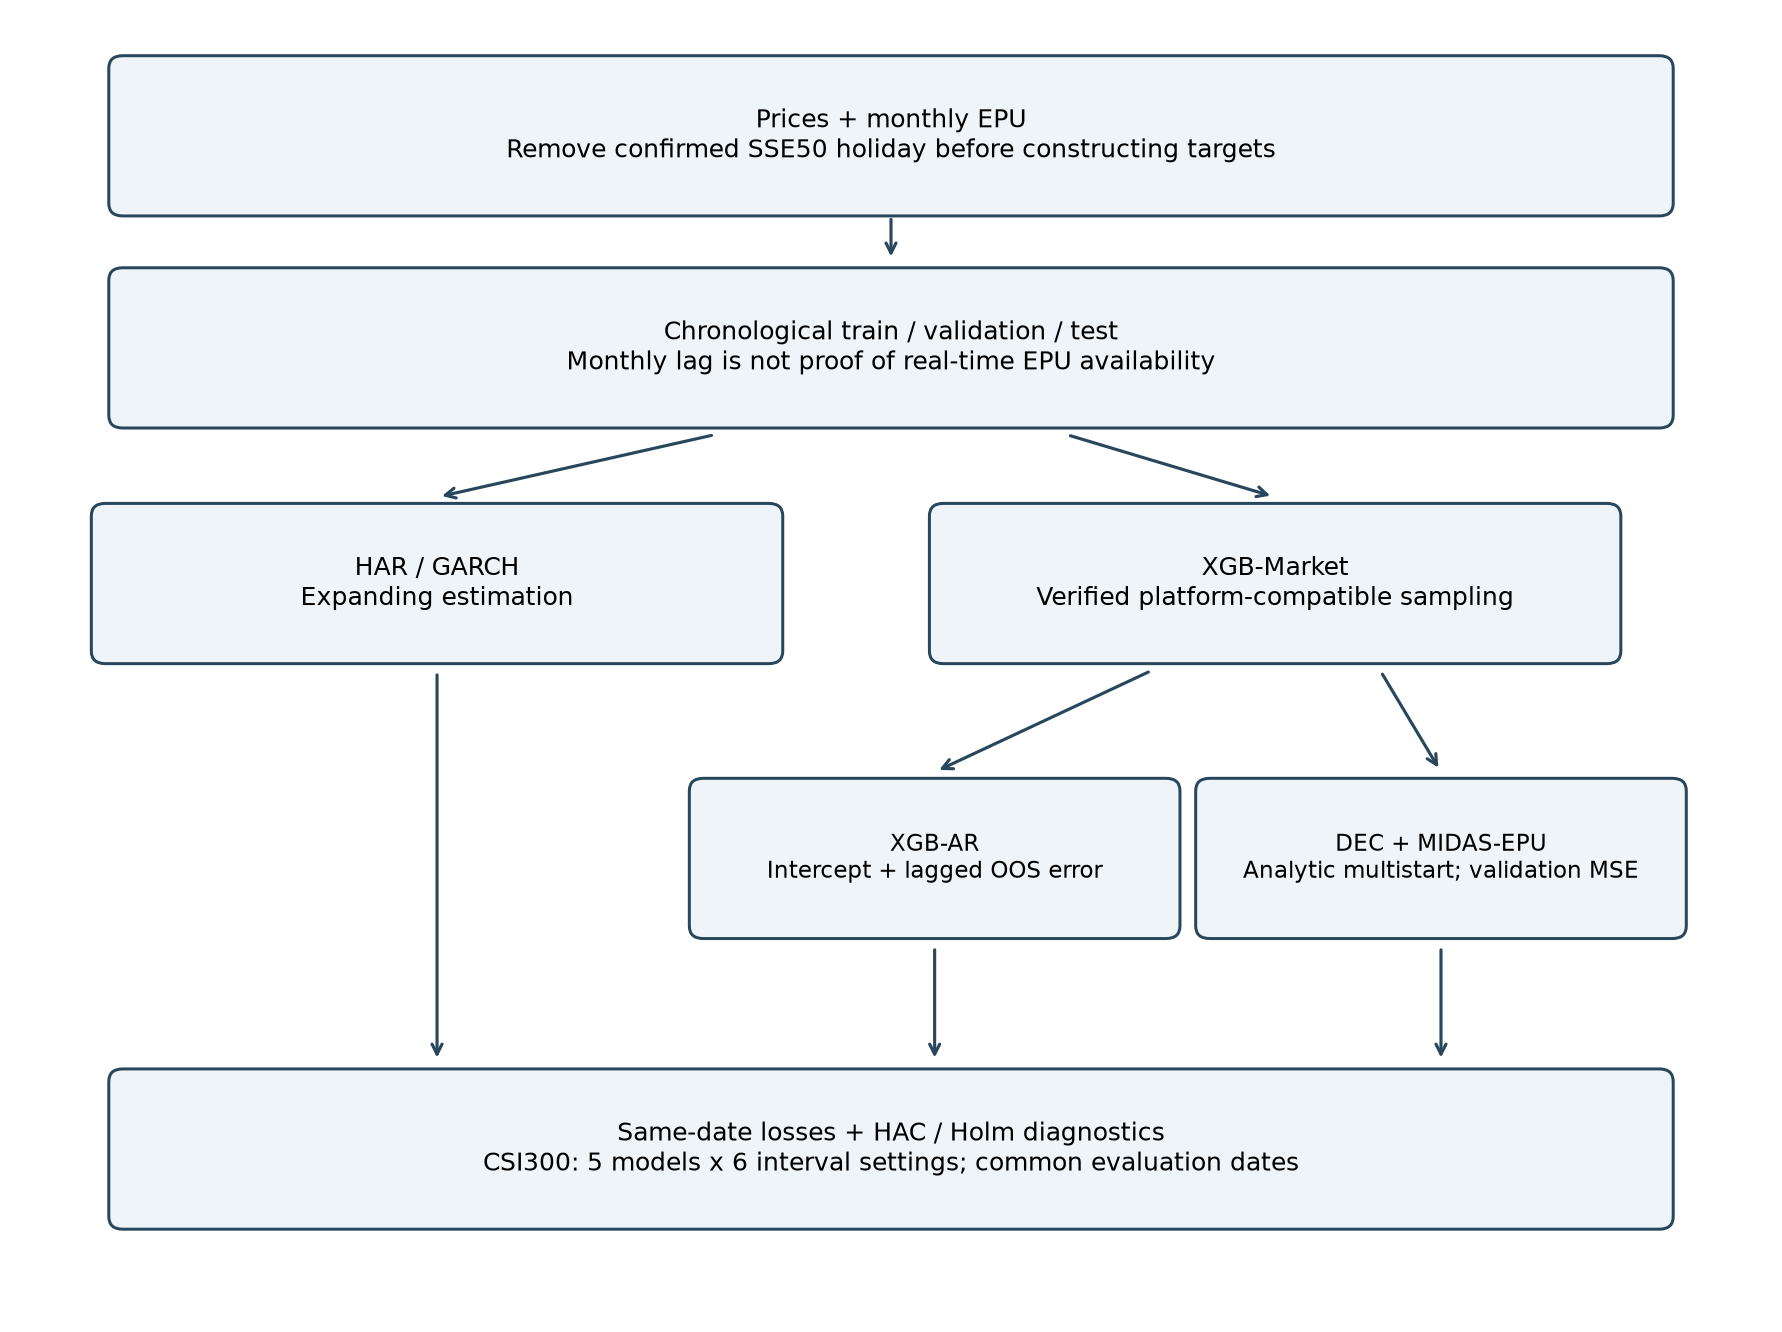
\includegraphics[width=\textwidth]{../../results/revised/method_flow.png}
\caption{Current workflow. Numerical checks, residual ablation, and common-date interval evaluation are separated from historical reproduction.}
\label{fig:f}
\end{figure}

Section~\ref{sec:methods} defines the data, models, estimation, and evaluation rules. Sections~\ref{sec:point} and~\ref{sec:intervals} report CSI300 point and interval results. Section~\ref{sec:robustness} examines SSE50 and Nasdaq. The conclusion and appendices state the reproducibility boundaries and historical controls.
\clearpage
